
%(BEGIN_QUESTION)
% Copyright 2008, Tony R. Kuphaldt, released under the Creative Commons Attribution License (v 1.0)
% This means you may do almost anything with this work of mine, so long as you give me proper credit

After the interior of this incinerator vessel is lined with brand-new refractory brick, it must be heated slowly to full temperature.  This slow heating process is called {\it curing}.  If heated too quickly, the steam pressure from the internal moisture in the brick cause the bricks to fracture or even explode.  The most important limit to observe in the initial act of curing the new refractory brick is not maximum temperature, but rather maximum temperature {\it rate}.

$$\includegraphics[width=15.5cm]{i0004rx01.eps}$$

If you were to observe the graph plotted by trend recorder TIR-36, what feature(s) of the graph would indicate to you the {\it rate} of temperature rise?  Be as specific as you can in your answer, giving a numerical example if possible.  Also, determine the unit of measurement for a temperature rate-of-change.

Also, identify the ISA tag letter used to represent an instrument measuring or acting upon the {\it rate-of-change} of some variable, and where you might install such an instrument in this system to help operations personnel monitor incinerator temperature rate.

\vskip 20pt \vbox{\hrule \hbox{\strut \vrule{} {\bf Suggestions for Socratic discussion} \vrule} \hrule}

\begin{itemize}
\item{} Describe how one would program a control system such as a DCS to calculate {\it rate} of temperature change to warn personnel working near the furnace if this rate becomes excessive.  Specifically, what mathematical steps must the control system do in order to calculate a rate-of-change value from successive temperature measurement values?
\end{itemize}

\underbar{file i01507}
%(END_QUESTION)





%(BEGIN_ANSWER)


%(END_ANSWER)





%(BEGIN_NOTES)

Calculating rate-of-change over time is as simple as calculating slope: {\it rise} over {\it run}.  In this case:

$$\hbox{Slope} = {dT \over dt}$$

If these slopes are hand-calculated between discrete points in time rather than calculated continuously by an analog computer, the actual equation is:

$$\hbox{Slope} = {\Delta T \over \Delta t}$$

The unit for rate-of-change is compound: unit of temperature over unit of time.  For example, degrees (either F or C) per minute.

\vskip 10pt

The ISA 5.1 standard reserves the letter ``K'' for rates of change.  Thus, this incinerator could be equipped with a temperature rate-of-change indicator called TKI-36.  Alarm units operating on the temperature rate-of-change would be labeled TKAH-36 (and possibly TKAL-36 if we were also concerned about high rates of temperature {\it fall} as well as high rates of temperature {\it rise}).














\vskip 20pt \vbox{\hrule \hbox{\strut \vrule{} {\bf Virtual Troubleshooting} \vrule} \hrule}

This question is a good candidate for a ``Virtual Troubleshooting'' exercise.  Presenting the diagram to students, you first imagine in your own mind a particular fault in the system.  Then, you present one or more symptoms of that fault (something noticeable by an operator or other user of the system).  Students then propose various diagnostic tests to perform on this system to identify the nature and location of the fault, as though they were technicians trying to troubleshoot the problem.  Your job is to tell them what the result(s) would be for each of the proposed diagnostic tests, documenting those results where all the students can see.

During and after the exercise, it is good to ask students follow-up questions such as:

\begin{itemize}
\item{} What does the result of the last diagnostic test tell you about the fault?
\item{} Suppose the results of the last diagnostic test were different.  What then would that result tell you about the fault?
\item{} Is the last diagnostic test the best one we could do?
\item{} What would be the ideal order of tests, to diagnose the problem in as few steps as possible?
\end{itemize}

%INDEX% Mathematics, calculus: rate of temperature rise
%INDEX% Process: incinerator (realistic P&ID shown)

%(END_NOTES)


